% LLM-CoNTM: Architecture & Training Flow
% Compile with: pdflatex llm_contm_flow.tex (requires TikZ, amsmath, booktabs)
\documentclass[11pt,a4paper]{article}

\usepackage{amsmath,amssymb,amsthm}
\usepackage{geometry}
\usepackage{booktabs}
\usepackage{xcolor}
\usepackage{hyperref}
\usepackage{algorithm}
\usepackage{algpseudocode}
\usepackage{tikz}
\usetikzlibrary{shapes.geometric, arrows.meta, positioning, fit, backgrounds, calc}
\usepackage{pgfplots}
\pgfplotsset{compat=1.18}

\geometry{margin=2.5cm}

\definecolor{colEncoder}{RGB}{52,120,196}
\definecolor{colDecoder}{RGB}{204,85,0}
\definecolor{colLoss}{RGB}{50,150,80}
\definecolor{colBuffer}{RGB}{160,50,180}
\definecolor{colGlobal}{RGB}{180,20,20}
\definecolor{colLocal}{RGB}{20,120,180}
\definecolor{colEMA}{RGB}{200,140,0}

\title{\textbf{LLM-CoNTM: LLM Embedding-based Continual Neural Topic Model}\\
\large Architecture, Loss Functions, and Streaming Training Flow}
\author{DCM-TM Extended Framework}
\date{May 2026}

\begin{document}
\maketitle
\tableofcontents
\newpage

% =============================================================================
\section{Overview}
% =============================================================================

LLM-CoNTM extends the Dirichlet-Categorical Mixture Topic Model (DCM-TM) by replacing the
standard bag-of-words decoder with an \textbf{LLM embedding-based ETM decoder}, and replacing
the classical online update rule with a \textbf{continual learning streaming loop} that employs:

\begin{enumerate}
  \item A \textbf{Dirichlet VAE encoder} (DVAE) mapping bag-of-words to topic proportions $\boldsymbol{\theta}$.
  \item A \textbf{frozen LLM word-embedding decoder} augmented by trainable local topic offsets
        and a non-linear gating module.
  \item A \textbf{tri-component loss}: ELBO + encoder distillation from LLM doc embeddings +
        contrastive decoder alignment.
  \item A \textbf{semantic memory buffer} for experience replay to prevent catastrophic forgetting.
  \item A \textbf{Target-Network-style EMA prior}: the global topic embedding tensor is frozen
        during gradient updates and updated once per timestamp via exponential moving average.
\end{enumerate}

\subsection{Data Flow Summary}

\[
  \underbrace{\text{BoW}(d)}_{\mathbb{R}^V}
  \;\xrightarrow{\text{DVAE Encoder}}\;
  (\boldsymbol{\mu}, \log\boldsymbol{\sigma}^2)
  \;\xrightarrow{\text{reparam.}}\;
  \underbrace{\boldsymbol{\theta}}_{\Delta^{K-1}}
  \;\xrightarrow{\text{ETM Decoder}}\;
  \underbrace{\log P(\mathbf{w}\mid d)}_{\mathbb{R}^V}
\]

\medskip
\noindent The decoder is conditioned on \emph{fused topic embeddings}:
\[
  \mathbf{T}_{\text{fused}} = \mathbf{T}_{\text{global}} + \mathbf{g} \odot \Delta\mathbf{T}_{\text{local}}
  \quad \in \mathbb{R}^{K \times D}
\]
where $\mathbf{T}_{\text{global}}$ is a frozen EMA buffer and $\Delta\mathbf{T}_{\text{local}}$
is the only decoder parameter touched by the optimizer.

% =============================================================================
\section{Preprocessing Pipeline}
% =============================================================================

\texttt{scripts/preprocess\_nips.py} produces all artifacts consumed by the training runner.
Figure~\ref{fig:preprocess} shows the stages.

\begin{figure}[h]
\centering
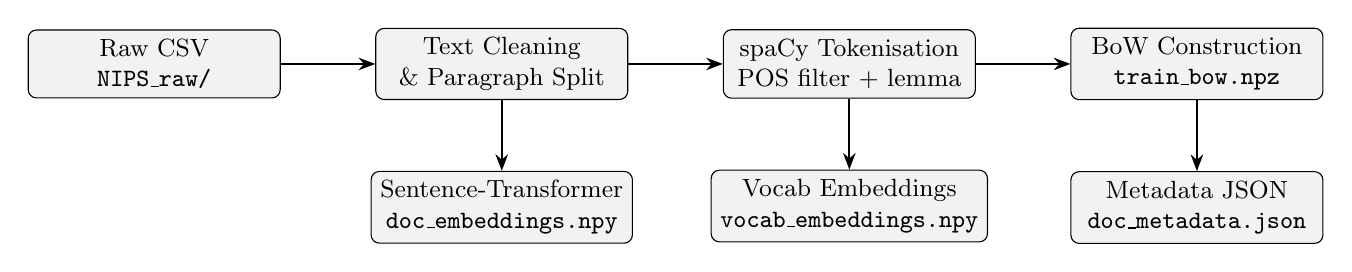
\begin{tikzpicture}[
  node distance=0.55cm and 0.3cm,
  box/.style={draw, rounded corners=3pt, minimum width=3.2cm, minimum height=0.75cm,
              fill=gray!10, font=\small, align=center},
  arr/.style={-{Stealth[length=6pt]}, thick},
]
  \node[box] (raw)    {Raw CSV\\\texttt{NIPS\_raw/}};
  \node[box, right=1.2cm of raw] (clean)  {Text Cleaning\\\& Paragraph Split};
  \node[box, right=1.2cm of clean] (spacy) {spaCy Tokenisation\\POS filter + lemma};
  \node[box, right=1.2cm of spacy] (bow)   {BoW Construction\\\texttt{train\_bow.npz}};
  \node[box, below=0.9cm of clean] (llmdoc) {Sentence-Transformer\\\texttt{doc\_embeddings.npy}};
  \node[box, below=0.9cm of spacy] (llmvoc) {Vocab Embeddings\\\texttt{vocab\_embeddings.npy}};
  \node[box, below=0.9cm of bow]   (meta)  {Metadata JSON\\\texttt{doc\_metadata.json}};

  \draw[arr] (raw)   -- (clean);
  \draw[arr] (clean) -- (spacy);
  \draw[arr] (spacy) -- (bow);
  \draw[arr] (clean.south) -- (llmdoc.north);
  \draw[arr] (spacy.south) -- (llmvoc.north);
  \draw[arr] (bow.south)   -- (meta.north);
\end{tikzpicture}
\caption{Preprocessing pipeline. Cleaning stage repairs hyphenated line breaks and
space-separated word fragments (e.g.\ ``alterna tives'' $\to$ ``alternatives'').
spaCy uses \texttt{en\_core\_web\_sm} with NOUN/VERB/ADJ/ADV POS filter and a suffix
blocklist to remove fragment tokens such as \emph{tion}, \emph{tive}, \emph{ment}.
Embeddings use \texttt{all-MiniLM-L6-v2} ($D=384$).}
\label{fig:preprocess}
\end{figure}

\paragraph{Output artefacts.}
\begin{center}
\begin{tabular}{lll}
\toprule
File & Shape & Description \\
\midrule
\texttt{train\_bow.npz}         & $(N_{\text{train}}, V)$ sparse & BoW counts, train split \\
\texttt{test\_bow.npz}          & $(N_{\text{test}}, V)$ sparse  & BoW counts, test split  \\
\texttt{doc\_embeddings.npy}    & $(N_{\text{total}}, 384)$      & LLM document embeddings \\
\texttt{vocab\_embeddings.npy}  & $(V, 384)$                     & LLM word embeddings (frozen anchor) \\
\texttt{vocab.txt}              & $V$ lines                      & Vocabulary list \\
\texttt{doc\_metadata.json}     & $N_{\text{total}}$ entries     & \texttt{\{ts, split\}} per document \\
\bottomrule
\end{tabular}
\end{center}

% =============================================================================
\section{Model Architecture}
% =============================================================================

\subsection{DVAE Encoder}

The encoder maps a normalised BoW vector to the parameters of a Log-Normal distribution
that approximates a Dirichlet prior (following AVITM / ProdLDA):

\begin{align}
  \hat{\mathbf{x}} &= \mathbf{x} \;/\; (\|\mathbf{x}\|_1 + \varepsilon) \label{eq:bow_norm}\\
  \mathbf{h}_1 &= \text{softplus}\!\left(\text{BN}_1(W_1 \,\text{drop}(\hat{\mathbf{x}}) + b_1)\right) \label{eq:enc_h1}\\
  \mathbf{h}_2 &= \text{softplus}\!\left(\text{BN}_2(W_2 \mathbf{h}_1 + b_2)\right) \label{eq:enc_h2}\\
  \boldsymbol{\mu} &= \text{BN}_\mu^{\text{no-aff}}(W_\mu \mathbf{h}_2 + b_\mu)
                    \in \mathbb{R}^K \label{eq:enc_mu}\\
  \log\boldsymbol{\sigma}^2 &= W_{\sigma} \mathbf{h}_2 + b_\sigma
                    \in \mathbb{R}^K \label{eq:enc_logvar}
\end{align}

\paragraph{Reparameterisation.}
\[
  \mathbf{z} = \boldsymbol{\mu} + \boldsymbol{\sigma} \odot \boldsymbol{\varepsilon},
  \quad \boldsymbol{\varepsilon} \sim \mathcal{N}(\mathbf{0}, \mathbf{I}),
  \qquad \boldsymbol{\theta} = \text{softmax}(\mathbf{z}) \in \Delta^{K-1}
\]

Hidden dimension: $H=256$. Dropout $p=0.2$.

\subsection{Non-Linear Gating Module}

The gating module fuses the global prior $\mathbf{T}_\text{global}$ and the local offset
$\Delta\mathbf{T}_\text{local}$ via a residual-gated structure inspired by GRU cells:

\begin{align}
  \mathbf{g} &= \sigma\!\left(W_z\,\Delta\mathbf{T}_\text{local} + b_z\right)
               \in (0,1)^{K \times D} \label{eq:gate}\\
  \mathbf{T}_\text{fused} &= \mathbf{T}_\text{global}
                             + \mathbf{g} \odot \Delta\mathbf{T}_\text{local}
               \in \mathbb{R}^{K \times D} \label{eq:fused}
\end{align}

The gate is driven solely by the local offset, so when $\Delta\mathbf{T}_\text{local} \to \mathbf{0}$
(start of a new timestamp), $\mathbf{T}_\text{fused} \approx \mathbf{T}_\text{global}$ and the
model defaults to the accumulated global prior.

\subsection{LLM Embedding Decoder}

Following the Embedded Topic Model (ETM), the decoder computes a topic-word distribution
$\boldsymbol{\beta}$ by matching topic embeddings against frozen LLM word embeddings $E \in \mathbb{R}^{V \times D}$:

\begin{align}
  \boldsymbol{\beta} &= \text{softmax}\!\left(
      \frac{\mathbf{T}_\text{fused}\, E^\top}{\tau}
    \right) \in \mathbb{R}^{K \times V} \label{eq:beta}\\
  \log P(\mathbf{w} \mid d) &= \log\!\left(\boldsymbol{\theta}\,\boldsymbol{\beta} + \varepsilon\right)
               \in \mathbb{R}^V \label{eq:recon}
\end{align}

where $\tau$ is a temperature hyperparameter (default $\tau = 1.0$).

\paragraph{Parameter roles.}
\begin{center}
\begin{tabular}{llll}
\toprule
Tensor & Shape & Type & Updated by \\
\midrule
$E$ (word embeddings) & $(V, D)$ & frozen buffer & never \\
$\mathbf{T}_\text{global}$ & $(K, D)$ & registered buffer & EMA only (after each timestamp) \\
$\Delta\mathbf{T}_\text{local}$ & $(K, D)$ & \texttt{nn.Parameter} & Adam optimizer \\
\bottomrule
\end{tabular}
\end{center}

\subsection{Full Architecture Diagram}

\begin{figure}[h]
\centering
\resizebox{\textwidth}{!}{%
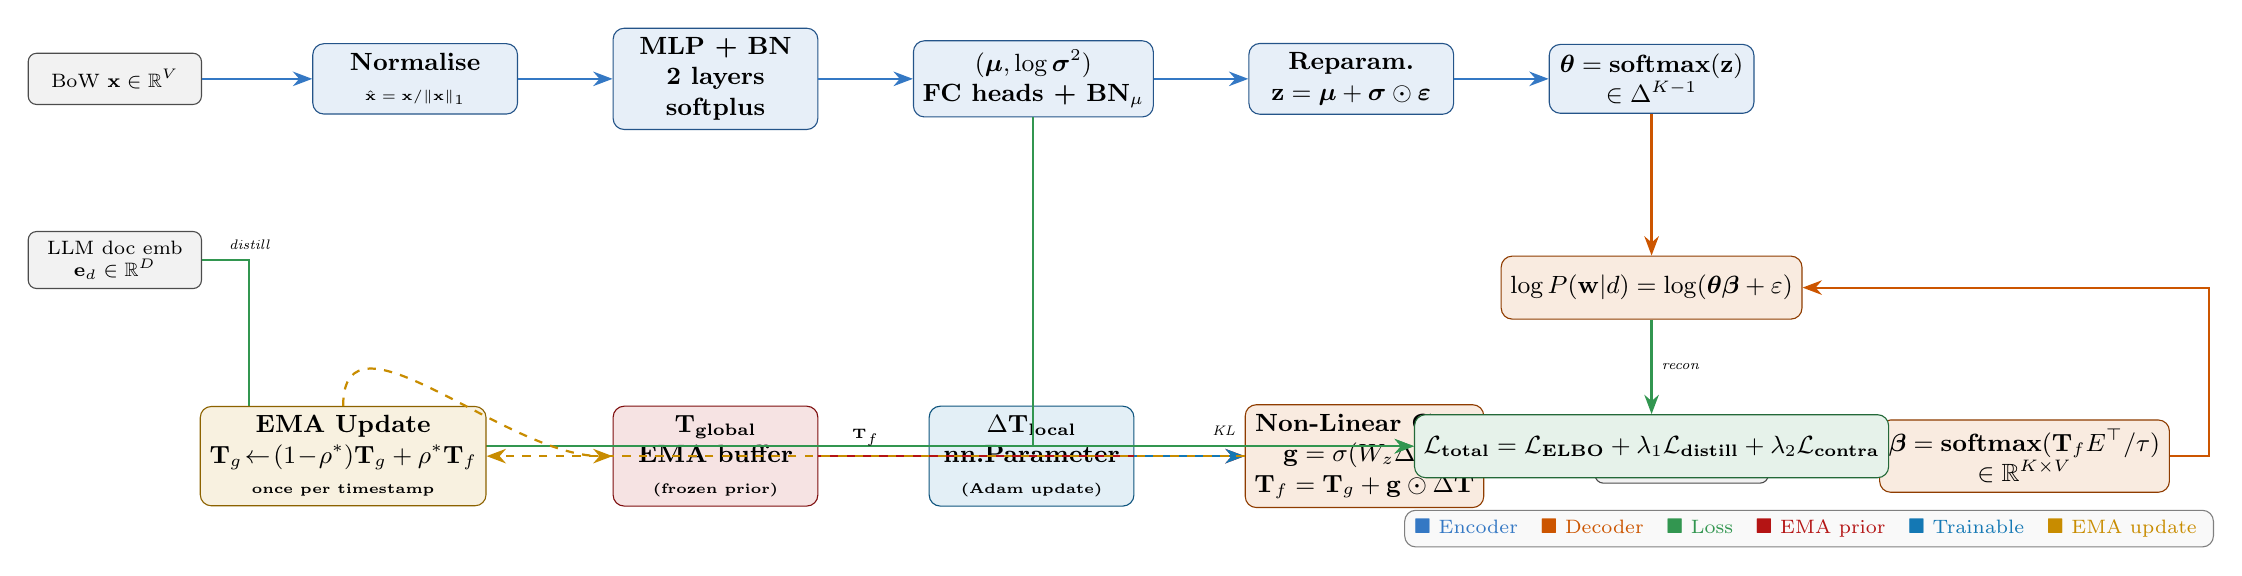
\begin{tikzpicture}[
  node distance=0.6cm and 0.7cm,
  block/.style={draw, rounded corners=4pt, minimum width=2.6cm, minimum height=0.8cm,
                fill=#1!12, draw=#1!70!black, font=\small\bfseries, align=center},
  smallblock/.style={draw, rounded corners=3pt, minimum width=2.2cm, minimum height=0.65cm,
                     fill=#1!10, draw=#1!60!black, font=\scriptsize, align=center},
  arr/.style={-{Stealth[length=7pt]}, thick, #1},
  label/.style={font=\scriptsize\itshape, #1},
]

% ─── INPUTS ───────────────────────────────────────────────────────────────────
\node[smallblock=gray] (bow_in)    at (0,0) {BoW $\mathbf{x}\in\mathbb{R}^V$};
\node[smallblock=gray, below=1.6cm of bow_in] (llm_in)  {LLM doc emb\\$\mathbf{e}_d\in\mathbb{R}^D$};

% ─── ENCODER ──────────────────────────────────────────────────────────────────
\node[block=colEncoder, right=1.4cm of bow_in] (norm)   {Normalise\\\tiny $\hat{\mathbf{x}}=\mathbf{x}/\|\mathbf{x}\|_1$};
\node[block=colEncoder, right=1.2cm of norm]   (mlp)    {MLP + BN\\2 layers\\softplus};
\node[block=colEncoder, right=1.2cm of mlp]    (muvar)  {$(\boldsymbol{\mu}, \log\boldsymbol{\sigma}^2)$\\FC heads + $\text{BN}_\mu$};
\node[block=colEncoder, right=1.2cm of muvar]  (reparam){Reparam.\\$\mathbf{z}=\boldsymbol{\mu}+\boldsymbol{\sigma}\odot\boldsymbol{\varepsilon}$};
\node[block=colEncoder, right=1.2cm of reparam](theta)  {$\boldsymbol{\theta}=\text{softmax}(\mathbf{z})$\\$\in\Delta^{K-1}$};

\draw[arr=colEncoder] (bow_in)  -- (norm);
\draw[arr=colEncoder] (norm)    -- (mlp);
\draw[arr=colEncoder] (mlp)     -- (muvar);
\draw[arr=colEncoder] (muvar)   -- (reparam);
\draw[arr=colEncoder] (reparam) -- (theta);

% ─── DECODER COMPONENTS ───────────────────────────────────────────────────────
\node[block=colGlobal, below=3.5cm of mlp]   (tglobal) {$\mathbf{T}_\text{global}$\\EMA buffer\\{\tiny(frozen prior)}};
\node[block=colLocal,  right=1.4cm of tglobal] (tlocal)  {$\Delta\mathbf{T}_\text{local}$\\nn.Parameter\\{\tiny(Adam update)}};
\node[block=colDecoder, right=1.4cm of tlocal]  (gate)    {Non-Linear Gate\\$\mathbf{g}=\sigma(W_z\Delta\mathbf{T})$\\$\mathbf{T}_f=\mathbf{T}_g+\mathbf{g}\odot\Delta\mathbf{T}$};
\node[smallblock=gray, right=1.4cm of gate] (wordEmb) {Word Emb $E$\\{\tiny frozen LLM}};
\node[block=colDecoder, right=1.4cm of wordEmb] (beta)    {$\boldsymbol{\beta}=\text{softmax}(\mathbf{T}_f E^\top/\tau)$\\$\in\mathbb{R}^{K\times V}$};

\draw[arr=colGlobal]  (tglobal) -- (gate);
\draw[arr=colLocal]   (tlocal)  -- (gate);
\draw[arr=gray]       (wordEmb) -- (beta);
\draw[arr=colDecoder] (gate)    -- node[above, label=black]{\tiny $\mathbf{T}_f$} (wordEmb);

% ─── ETM COMBINE ──────────────────────────────────────────────────────────────
\node[block=colDecoder, below=1.8cm of theta] (etm) {$\log P(\mathbf{w}|d)=\log(\boldsymbol{\theta}\boldsymbol{\beta}+\varepsilon)$};

\draw[arr=colDecoder] (theta.south) -- (etm.north);
\draw[arr=colDecoder] (beta.east) -| ++(0.5,0) |- (etm.east);

% ─── LOSS ─────────────────────────────────────────────────────────────────────
\node[block=colLoss, below=1.2cm of etm] (loss) {$\mathcal{L}_\text{total}=\mathcal{L}_\text{ELBO}+\lambda_1\mathcal{L}_\text{distill}+\lambda_2\mathcal{L}_\text{contra}$};

\draw[arr=colLoss] (etm.south) -- node[right, label=black]{\tiny recon} (loss.north);
\draw[arr=colLoss] (muvar.south) |- node[near end, above, label=black]{\tiny KL} (loss.west);
\draw[arr=colLoss] (llm_in.east) -| node[near end, above, label=black]{\tiny distill} ++(0.6,0) |- (loss.west);

% ─── EMA UPDATE ───────────────────────────────────────────────────────────────
\node[block=colEMA, left=1.6cm of tglobal] (ema) {EMA Update\\$\mathbf{T}_g\!\leftarrow\!(1\!-\!\rho^*)\mathbf{T}_g+\rho^*\mathbf{T}_f$\\{\tiny once per timestamp}};

\draw[arr={colEMA, dashed}] (gate.west) to[out=180, in=0] node[above, label=black]{\tiny $\mathbf{T}_f$} (ema.east);
\draw[arr={colEMA, dashed}] (ema.north) to[out=90, in=180] (tglobal.west);

% ─── LEGEND BOX ───────────────────────────────────────────────────────────────
\node[draw=gray, rounded corners, fill=gray!5, font=\scriptsize, align=left,
      below=0.4cm of loss, xshift=2cm] (legend) {
  \textcolor{colEncoder}{$\blacksquare$ Encoder}~~
  \textcolor{colDecoder}{$\blacksquare$ Decoder}~~
  \textcolor{colLoss}{$\blacksquare$ Loss}~~
  \textcolor{colGlobal}{$\blacksquare$ EMA prior}~~
  \textcolor{colLocal}{$\blacksquare$ Trainable}~~
  \textcolor{colEMA}{$\blacksquare$ EMA update}
};

\end{tikzpicture}
}
\caption{LLM-CoNTM architecture. Solid arrows: gradient-enabled forward pass.
Dashed arrows: \texttt{@torch.no\_grad()} EMA update, executed once after each
timestamp's training loop completes.}
\label{fig:arch}
\end{figure}

% =============================================================================
\section{Loss Functions}
% =============================================================================

\subsection{ELBO (Evidence Lower Bound)}

Standard DVAE ELBO with KL annealing coefficient $w_\text{KL} \in [0,1]$:

\begin{align}
  \mathcal{L}_\text{ELBO}
  &= \underbrace{-\mathbb{E}_{q}\!\left[\sum_{w} x_w \log P(w \mid \boldsymbol{\theta})\right]}_{\mathcal{L}_\text{recon}}
   + \; w_\text{KL}\,\underbrace{D_\text{KL}\!\left[q(\boldsymbol{\theta}\mid\mathbf{x}) \,\|\, p(\boldsymbol{\theta})\right]}_{\mathcal{L}_\text{KL}} \label{eq:elbo}
\end{align}

Under the Log-Normal approximation the KL term has the closed form:
\[
  \mathcal{L}_\text{KL} = -\tfrac{1}{2}\sum_{k=1}^{K}
    \left(1 + \log\sigma_k^2 - \mu_k^2 - \sigma_k^2\right)
\]

KL annealing: $w_\text{KL} = \min\!\left(1,\, \frac{e}{E_\text{warmup}}\right)$
with $E_\text{warmup}=20$ epochs.

\subsection{Encoder Distillation Loss}

Aligns the encoder's predicted topic distribution with the LLM's semantic
understanding of the document:

\begin{align}
  \tilde{\boldsymbol{\theta}}_\text{teacher}
    &= \text{softmax}\!\left(\frac{W_s\,\mathbf{e}_d}{\tau}\right) \in \Delta^{K-1}
    \label{eq:teacher}\\
  \mathcal{L}_\text{distill}
    &= D_\text{KL}\!\left[\tilde{\boldsymbol{\theta}}_\text{teacher}
                          \;\|\; \boldsymbol{\theta}\right]
     = \sum_k \tilde{\theta}_k \log\frac{\tilde{\theta}_k}{\theta_k}
    \label{eq:distill}
\end{align}

where $W_s \in \mathbb{R}^{K \times D}$ is a learned linear projection
(\texttt{distill\_proj}), and $\mathbf{e}_d \in \mathbb{R}^D$ is the LLM
embedding of document $d$.

\subsection{Contrastive Decoder Loss}

Pulls topic embeddings towards their highest-probability words and
pushes them away from the rest of the vocabulary:

\begin{align}
  \mathcal{L}_\text{contra}
  &= -\frac{1}{K}\sum_{k=1}^{K}
     \left[
       \log\sum_{w \in \mathcal{W}_k} \exp\!\left(\frac{\mathbf{T}_k^\top \mathbf{e}_w}{\tau}\right)
       - \log\sum_{w' \in \mathcal{V}} \exp\!\left(\frac{\mathbf{T}_k^\top \mathbf{e}_{w'}}{\tau}\right)
     \right]
  \label{eq:contra}
\end{align}

where $\mathcal{W}_k = \operatorname{Top-N}(\boldsymbol{\beta}_{k,\cdot})$ are the
$N=20$ words with the highest probability under topic $k$, computed from a
detached copy of $\boldsymbol{\beta}$.

\subsection{Total Loss}

\begin{equation}
  \boxed{
    \mathcal{L}_\text{total}
    = \mathcal{L}_\text{ELBO}
    + \lambda_1 \mathcal{L}_\text{distill}
    + \lambda_2 \mathcal{L}_\text{contra}
  }
  \label{eq:total}
\end{equation}

Default: $\lambda_1 = \lambda_2 = 0.1$.

% =============================================================================
\section{Semantic Memory Buffer}
% =============================================================================

The \texttt{SemanticMemoryBuffer} prevents catastrophic forgetting by storing
a diverse reservoir of past documents that are replayed during training on new timestamps.

\paragraph{Diversity score.}
For each candidate document with LLM embedding $\mathbf{e}$:
\[
  u(\mathbf{e}) = 1 - \max_{j \in \text{buffer}} \cos(\mathbf{e},\, \mathbf{e}_j)
\]
A score of 1 means the document is entirely novel; 0 means it is a duplicate.

\paragraph{Admission policy.}
\begin{itemize}
  \item If buffer size $< M_{\max}$: admit unconditionally.
  \item If full: replace the least-unique stored document iff $u(\mathbf{e}) > u_{\min}$.
\end{itemize}

\paragraph{Sampling.}
$n$ documents are sampled without replacement, with probability proportional to uniqueness:
$p_j \propto u(\mathbf{e}_j)$.

\paragraph{Replay interleaving.}
During each batch step, $\lfloor r \cdot B \rfloor$ replay documents are prepended
(default ratio $r=0.2$, batch size $B=256$). The combined batch is normalised BoW
before being passed to the encoder.

% =============================================================================
\section{Adaptive Plasticity: Semantic Surprise Index}
% =============================================================================

\subsection{Surprise Index $\eta_t$}

The surprise index quantifies how semantically different the current timestamp's
data is from the previous one:

\begin{equation}
  \eta_t = 1 - \cos\!\left(\bar{\mathbf{h}}_t,\, \bar{\mathbf{h}}_{t-1}\right),
  \qquad \eta_t \in [0, 2]
  \label{eq:surprise}
\end{equation}

where $\bar{\mathbf{h}}_t$ is the mean (L2-normalised) LLM embedding of the
current mini-batch. $\eta_0 = 0.5$ (default).

\subsection{Adaptive EMA Rate $\rho_t^*$}

\begin{align}
  \rho_t &= \frac{1}{(\tau_0 + t)^\kappa} & &\text{(polynomial decay baseline)} \\
  \rho_t^* &= \min\!\left(\rho_t \cdot (1 + \gamma\,\eta_t),\; 0.95\right)
              & &\text{(surprise-amplified, capped)} \label{eq:rho_star}
\end{align}

Default: $\gamma=2.0$, $\tau_0=1.0$, $\kappa=0.7$.
High surprise $\Rightarrow$ larger EMA step; low surprise $\Rightarrow$ conservative update.

% =============================================================================
\section{Target-Network EMA Prior Update}
% =============================================================================

Inspired by the \emph{Target Network} in DQN and \emph{Mean Teacher} in
semi-supervised learning, the global topic embedding tensor is treated as a
\textbf{frozen prior} during the gradient-update phase. It is updated exactly
\emph{once per timestamp}, after the full training loop has converged:

\begin{equation}
  \boxed{
    \mathbf{T}_\text{global}^{(t+1)}
    \;\leftarrow\;
    (1 - \rho_t^*)\,\mathbf{T}_\text{global}^{(t)}
    \;+\;
    \rho_t^*\,\mathbf{T}_\text{fused}^{(t)}
  }
  \label{eq:ema}
\end{equation}

where $\mathbf{T}_\text{fused}^{(t)} = \mathbf{T}_\text{global}^{(t)} +
\mathbf{g}^{(t)} \odot \Delta\mathbf{T}_\text{local}^{(t)}$ is computed
at the \emph{best-checkpoint} state restored after training.

\paragraph{Implementation.} \texttt{topic\_embeddings\_global} is a
\texttt{register\_buffer} (not an \texttt{nn.Parameter}), so it is
\emph{invisible to the optimizer} and moves with \texttt{.to(device)} correctly.
The update is performed inside \texttt{model.ema\_update\_global(rho\_star)}
decorated with \texttt{@torch.no\_grad()}.

\paragraph{Contrast with intra-batch updates.} In previous designs, EMA was
applied on every mini-batch (Step F inside \texttt{train\_streaming\_step}).
The new design removes Step~F from the batch loop entirely, making the global
prior \emph{stable} for the duration of each timestamp's training — analogous
to how word embeddings are frozen in standard fine-tuning.

% =============================================================================
\section{Streaming Training Loop}
% =============================================================================

Algorithm~\ref{alg:streaming} describes the full pipeline.

\begin{algorithm}[h]
\caption{LLM-CoNTM Streaming Training Pipeline}
\label{alg:streaming}
\begin{algorithmic}[1]
\Require Timestamps $\{T_0, T_1, \dots, T_{S-1}\}$, word embeddings $E$ (frozen),
         config $\Theta$
\State Initialise $\mathbf{T}_\text{global} \sim \mathcal{N}(\mathbf{0}, 0.02^2\mathbf{I})$,
       $\Delta\mathbf{T}_\text{local} = \mathbf{0}$, buffer $\mathcal{B} = \emptyset$

\For{$t = 0, 1, \dots, S-1$}

  \If{$t > 0$}
    \State $\Delta\mathbf{T}_\text{local} \leftarrow \mathbf{0}$ \Comment{Reset local offsets}
  \EndIf

  \State Build \texttt{DataLoader} for $\mathcal{D}_t^{\text{train}}$ (drop\_last=True)

  \For{epoch $e = 1 \dots E_{\max}$}
    \State $w_\text{KL} = \min(1,\; e / E_{\text{warm}})$
    \For{each mini-batch $(\mathbf{X}, \mathbf{E}_d) \in \mathcal{D}_t^{\text{train}}$}
      \State Prepend $\lfloor r|\mathbf{X}|\rfloor$ replay samples from $\mathcal{B}$
      \State $\eta_t \leftarrow \textsc{SurpriseIndex}(\mathbf{E}_d, \bar{\mathbf{h}}_{t-1})$
             \Comment{Eq.~\ref{eq:surprise}}
      \State Forward: $\boldsymbol{\theta}, \mathbf{T}_\text{fused}, \boldsymbol{\beta}
             \leftarrow \textsc{Model}(\mathbf{X}, E, w_\text{KL})$
      \State $\mathcal{L} \leftarrow \mathcal{L}_\text{ELBO} + \lambda_1\mathcal{L}_\text{distill}
             + \lambda_2\mathcal{L}_\text{contra}$ \Comment{Eq.~\ref{eq:total}}
      \State \textbf{Backprop} and \textbf{Adam step} on $\{\Delta\mathbf{T}_\text{local},
             \text{encoder}, W_s\}$ only
      \State $\mathcal{B}.\textsc{AddBatch}(\mathbf{X}, \mathbf{E}_d)$
             \Comment{Diversity-based reservoir}
      \State $\bar{\mathbf{h}}_{t} \leftarrow \bar{\mathbf{h}}_{\text{batch}}$
    \EndFor
    \State LR scheduler step (ReduceLROnPlateau)
  \EndFor

  \State Restore best-checkpoint (lowest epoch loss) \label{alg:restore}
  \State $\rho_t^* \leftarrow \textsc{AdaptiveRate}(t, \eta_t)$
         \Comment{Eq.~\ref{eq:rho_star}}
  \State $\mathbf{T}_\text{global} \leftarrow
         (1-\rho_t^*)\mathbf{T}_\text{global} + \rho_t^*\mathbf{T}_\text{fused}$
         \Comment{EMA update, Eq.~\ref{eq:ema}, once only}
  \State Extract $\boldsymbol{\beta}$, compute topics $\mathcal{T}_t$, save checkpoint
\EndFor

\State Save final topics to \texttt{final\_global\_memory/}, run \texttt{evaluation.py}
\end{algorithmic}
\end{algorithm}

% =============================================================================
\section{Evaluation Metrics}
% =============================================================================

After training all timestamps, \texttt{scripts/evaluation.py} loads
\texttt{final\_global\_memory/} and computes:

\paragraph{Topic Diversity (TD).}
\[
  \text{TD} = \frac{|\text{unique words in top-}M\text{ lists across all }K\text{ topics}|}{M \cdot K}
  \in [0, 1]
\]
Higher is better; $M=15$ words per topic by default.

\paragraph{Normalised PMI Coherence (NPMI).}
\[
  \text{NPMI}(k) = \frac{2}{N(N-1)}\sum_{i<j}
  \frac{\log\frac{P(w_i,w_j) + \varepsilon}{P(w_i)P(w_j)}}
       {-\log(P(w_i,w_j) + \varepsilon)}
\]
where co-occurrence probabilities are estimated over the training corpus.
Averaged over all $K$ topics; range $[-1, 1]$, higher is better.

% =============================================================================
\section{Hyperparameter Summary}
% =============================================================================

\begin{center}
\begin{tabular}{llll}
\toprule
Parameter & Symbol & Default & Role \\
\midrule
Topics           & $K$               & 50    & Number of latent topics \\
Embedding dim    & $D$               & 384   & LLM embedding dimension \\
Encoder hidden   & $H$               & 256   & MLP hidden width \\
Dropout          & $p$               & 0.2   & Encoder dropout \\
Temperature      & $\tau$            & 1.0   & ETM and distill softmax \\
Distillation wt  & $\lambda_1$       & 0.1   & Weight for $\mathcal{L}_\text{distill}$ \\
Contrastive wt   & $\lambda_2$       & 0.1   & Weight for $\mathcal{L}_\text{contra}$ \\
Learning rate    & $\alpha$          & 0.002 & Adam base LR \\
Batch size       & $B$               & 256   & Mini-batch size \\
Epochs / ts      & $E_\text{max}$    & 80    & Epochs per timestamp \\
KL warmup        & $E_\text{warm}$   & 20    & KL annealing epochs \\
Replay ratio     & $r$               & 0.2   & Fraction of batch from replay \\
Buffer size      & $M_\text{max}$    & 500   & Max documents in memory \\
Surprise amplify & $\gamma$          & 2.0   & EMA rate amplification \\
Decay base       & $\tau_0$          & 1.0   & Polynomial decay offset \\
Decay exponent   & $\kappa$          & 0.7   & Polynomial decay exponent \\
Top-N contrastive& $N$               & 20    & Top words for contrastive loss \\
\bottomrule
\end{tabular}
\end{center}

% =============================================================================
\section{File Structure}
% =============================================================================

\begin{verbatim}
DCM-TM/
├── run_llm_contm.py              Main runner: streaming pipeline, evaluation
├── src/
│   ├── llm_contm.py              Model, losses, memory buffer, streaming step
│   │   ├── DVAEEncoder             BoW → (μ, log σ²) → θ
│   │   ├── NonLinearGatingModule   Gate fusion of global + local embeddings
│   │   ├── LLMEmbeddingDecoder     ETM decoder with EMA buffer
│   │   ├── LLMEncoderDecoderCoNTM  Full model (encoder + decoder + EMA)
│   │   ├── CoNTMTotalLoss          ELBO + distillation + contrastive
│   │   ├── SemanticMemoryBuffer    Diversity-based experience replay
│   │   ├── train_streaming_step()  Per-batch training step with replay
│   │   ├── compute_surprise_index()  η_t = 1 − cos(H_t, H_{t−1})
│   │   ├── compute_adaptive_lr_scale()  ρ*_t with surprise amplification
│   │   └── update_global_embeddings_ema()  EMA utility (standalone)
│   ├── global_memory.py          GlobalMemory class (evaluation compat.)
│   ├── topic_utils.py            TD, NPMI, extract_topics, embed_topics
│   └── vae.py                    Original ProdLDA (unchanged)
├── scripts/
│   ├── preprocess_nips.py        Full preprocessing pipeline
│   └── evaluation.py             TD + NPMI from final_global_memory/
├── data/
│   └── NIPS/                     Preprocessed artifacts
│       ├── train_bow.npz
│       ├── doc_embeddings.npy    (N_total, 384)
│       ├── vocab_embeddings.npy  (V, 384)  — frozen word embeddings
│       ├── vocab.txt
│       └── doc_metadata.json
└── outputs_llm_contm/
    ├── T0/ … T10/                Per-timestamp checkpoints
    └── final_global_memory/      Final topics for evaluation
\end{verbatim}

\end{document}
